\section{Uživatelské rozhraní}
V této kapitole se pokusím vysvětlit, jak používat aplikaci, jak se ovládá a co se s ní dá dělat. Dále uvedu příklady mnou vytvořených časových os. 

\subsection{Navigace na stránce}
Stránka používá k navigaci horní lištu se záložkami jednotlivých sekcí stránek (tento prvek je uložen jako \textit{default.vue} ve složce \textit{layout}). Na menších zařízeních se místo záložek objeví rozklikávací menu pro výběr jednotlivých stránek.

\begin{figure}[h]
    \centering
    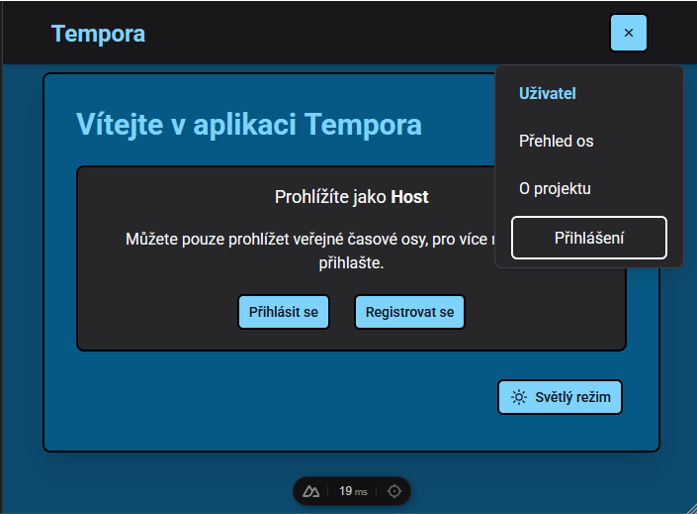
\includegraphics[width=0.6\linewidth]{Images/Mobile.png}
    \caption{Mobilní rozhraní ve tmavém režimu}
    \label{fig:mobile}
\end{figure}

\subsection{Tvorba osy}
Pokud je uživatel registrován a přihlášen, může vytvořit vlastní časovou osu. Nejprve se musí přesunout do sekce „Přehled os“, kde se nachází vybrané osy, osy vytvořené uživatelem a uložené osy, viz obrázek \ref{fig:LineHub}. V této sekci lze také vyhledávat osy podle jejich ID nebo celého odkazu. 

\begin{figure}[h]
    \centering
    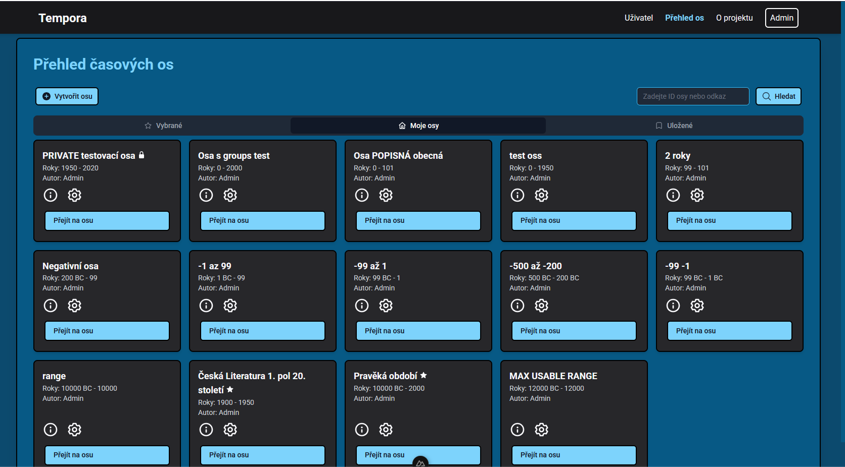
\includegraphics[width=0.8\linewidth]{Images/LineHub.png}
    \caption{Stránka Přehled os (tmavý režim)}
    \label{fig:LineHub}
\end{figure}

Po kliknutí na tlačítko „Vytvořit osu“ se otevře nová nabídka, kam uživatel zadává jméno časové osy, rok začátku a konce popisovaného období (pro zadání let před naším letopočtem se používá znak mínus před počtem let) a krátký popis dané osy, který může obsahovat například zdroje, odkud čerpal při tvorbě.

Na pravé straně je možnost pojmenovat jednotlivé řádky. Také lze nastavit osu jako soukromou, což znemožní komukoliv kromě autora si tuto osu zobrazit.

\begin{figure}[h]
    \centering
    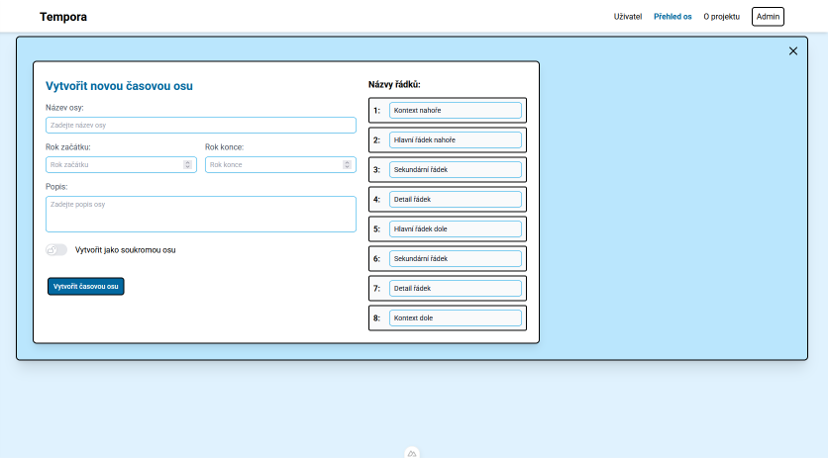
\includegraphics[width=0.8\linewidth]{Images/CreateNew.png}
    \caption{Tvorba nové osy (světlý režim)}
    \label{fig:CreateNew}
\end{figure}

\subsection{Ovládání osy}
Po vytvoření osy je uživatel přesunut přímo na stránku, kde se daná osa zobrazuje. Zde se nachází časová osa, uprostřed níž jsou uváděny letopočty. Pod osou je ovládací panel, pomocí kterého se osa posouvá, přibližuje nebo oddaluje. Nachází se zde také prvek, který ukazuje letopočet odpovídající pozici červené čáry a kurzoru umístěného na časové ose pro lepší orientaci. 

Klíčovou roli v ovládání má postranní lišta napravo, obsahující tlačítka: informace o ose, zapnutí editačního režimu, sdílení, nastavení, uložení, přidání nové události a přepnutí světlého/tmavého režimu.
\newpage

Na obrázku \ref{fig:AuthorTimeline} je zapnutý editační režim, což znamená, že po kliknutí na jednotlivé události je můžete upravovat. Zároveň se objeví nové tlačítko pro přidání události (více v sekci \ref{Úprava událostí} Úprava událostí). Tlačítko pro přepnutí časové osy do tmavého/světlého režimu funguje nezávisle na režimu celé aplikace a umožňuje uživateli zachovat jeho preferovaný režim, přičemž osu zobrazí v režimu, který se mu bude zdát příjemnější. 

Celou boční lištu lze také sbalit, aby nepřekážela. Pokud si prohlížíte osu, jejímž autorem nejste, uvidíte boční lištu tak, jak je zobrazena na obrázku \ref{fig:GuestTimeline}.


\begin{figure}[h]
    \centering
    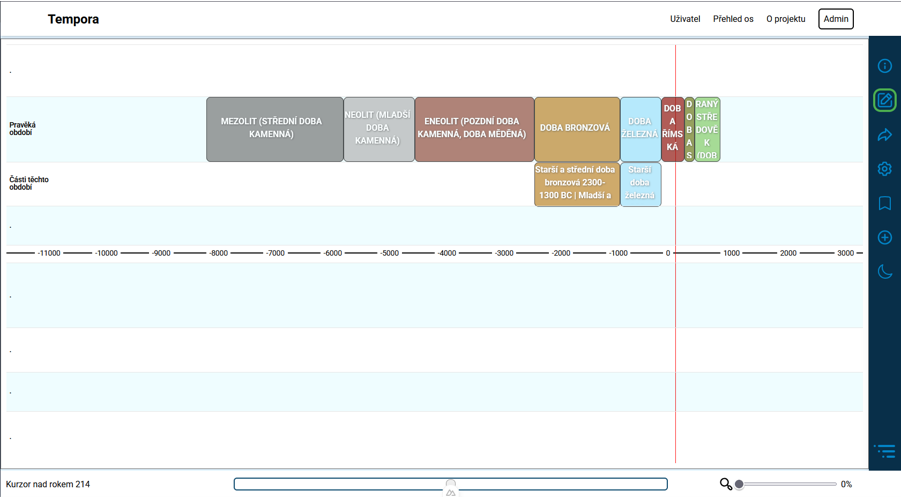
\includegraphics[width=0.8\linewidth]{Images/AuthorTimeline.png}
    \caption{Zobrazení postranní lišty - autor (světlí režim osy)}
    \label{fig:AuthorTimeline}
\end{figure}

\begin{figure}[h]
    \centering
    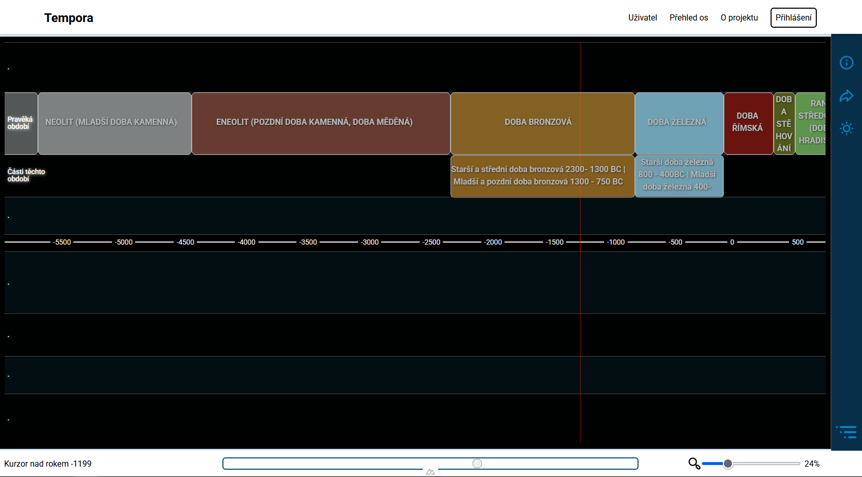
\includegraphics[width=0.8\linewidth]{Images/GuestTimeline.png}
    \caption{Zobrazení postranní lišty - návštěvník (tmavý režim osy)}
    \label{fig:GuestTimeline}
\end{figure}

\newpage

\subsection{Přidání a úprava události}
\label{Úprava událostí}
Pro přidání nové události musí být autor dané osy v editačním režimu a kliknout na tlačítko „Přidat událost“ (+), což ho přesměruje na URL nové události, kterou může začít upravovat, viz obrázek \ref{fig:NewItem}. 

V horní části si může vybrat, jestli chce vytvořit kontextovou nebo hlavní událost. Obě tyto části potřebují zadat roky trvání, aby se mohly na časovou osu umístit, a jejich zobrazované jméno, případně popis. Dále si také může vybrat, jakou barvu bude událost mít na časové ose – tato barva dynamicky mění okraj události. Pokud si uživatel zvolí hlavní událost, dostane možnost přidání vedlejší části a části detailu. Každá část umožňuje použít panel nástrojů pro editaci podrobností textu, odkazů, vzorců nebo zarovnání paragrafu. 

\begin{figure}[h]
    \centering
    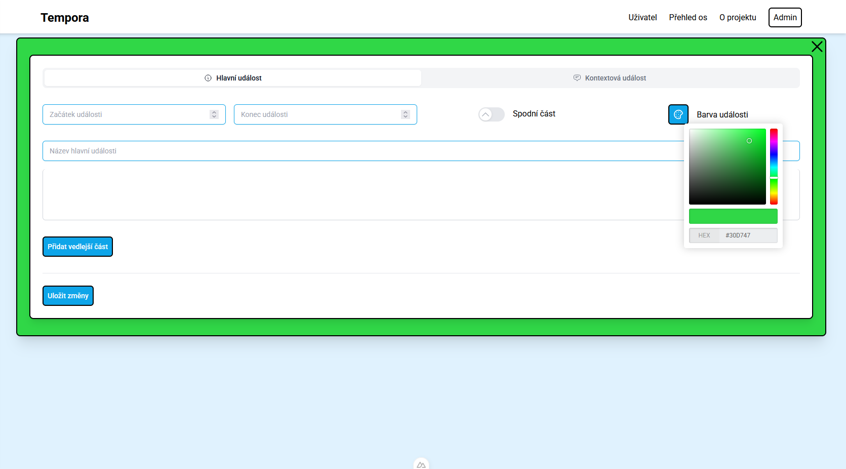
\includegraphics[width=0.8\linewidth]{Images/NewItem.png}
    \caption{Tvorba nové události}
    \label{fig:NewItem}
\end{figure}

Pokud chce uživatel upravit již vytvořenou událost, musí mít zapnutý editační režim a kliknout na událost na časové ose, kterou chce změnit. Otevře se mu stejné menu jako při tvorbě nové události, ale s načteným obsahem z databáze. Jedinou změnou je, že si nevybírá mezi hlavní a kontextovou událostí a může zahodit změny, které provedl, nebo smazat celou událost.  

\begin{figure}[h]
    \centering
    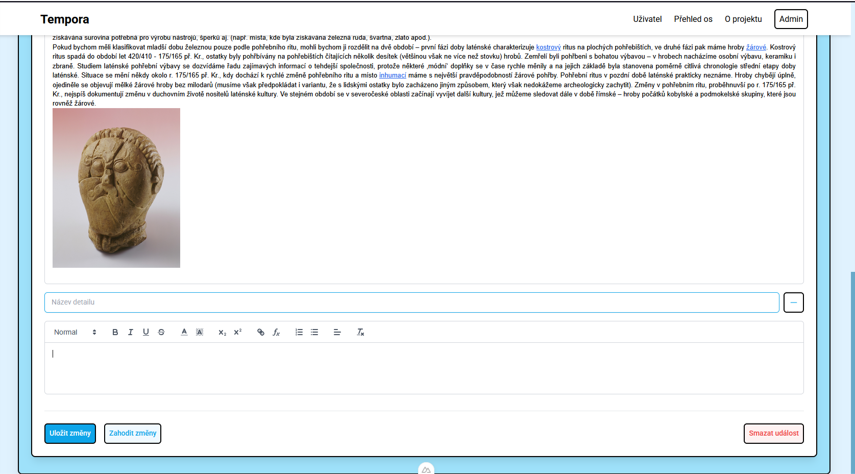
\includegraphics[width=0.8\linewidth]{Images/EditItem.png}
    \caption{Úprava již vytvořené události}
    \label{fig:EditItem}
\end{figure}


\subsection{Zobrazení události}
Pokud si chce uživatel prohlédnout podrobnosti o události, musí vypnout editační režim a kliknout na danou událost na časové ose. Poté se zobrazí stránka, na které jsou části rozděleny přesně podle toho, jak byly vytvořeny – s hlavním nadpisem a roky trvání. Pokud je vytvořeno více hlavních událostí v tomto řádku, objeví se nahoře také šipky pro přesměrování, ukazující, které období předcházelo a které následuje. 

\begin{figure}[h]
    \centering
    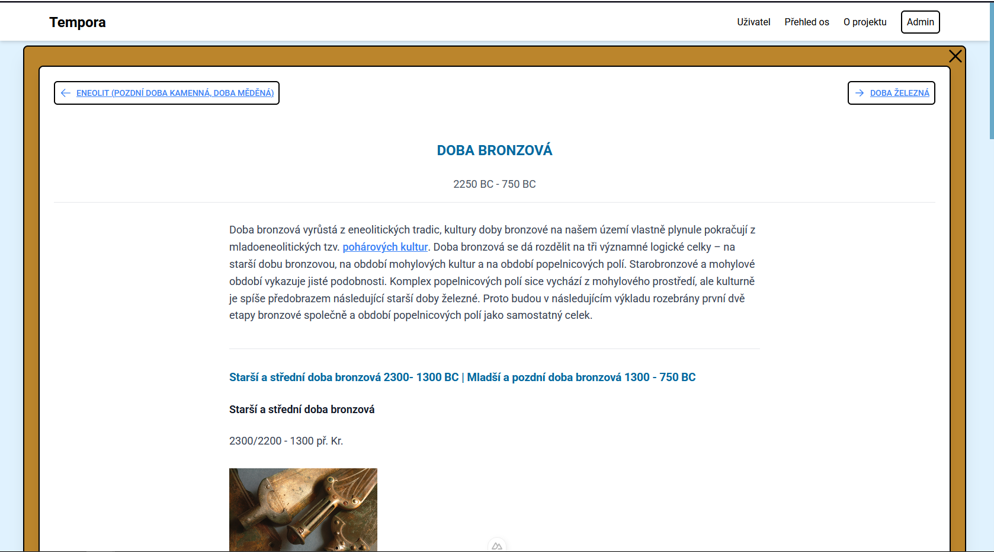
\includegraphics[width=0.8\linewidth]{Images/showItem.png}
    \caption{Ukázka zobrazení podrobností o události}
    \label{fig:showItem}
\end{figure}


\subsection{Vylepšení uživatelské zkušenosti}
Jedním z mých hlavních cílů bylo vytvořit uživatelsky příjemné a intuitivní prostředí. Proto jsem se již od začátku snažil tvořit prvky pro zpětnou vazbu – tlačítka změní barvu, když na ně najedete kurzorem, při načítání dat z databáze je vypsán aktuální stav toho, co se právě děje, a smazání údajů se nestane omylem díky potvrzovacímu dialogu. Celá webová aplikace podporuje světlý i tmavý režim (pomocí \textit{Tailwind} \texttt{dark:}), a časová osa má svůj vlastní přepínač, aby se zabránilo špatně vypadajícím barvám v jednom z režimů. 

Aplikace často využívá ikony z knihovny \textit{Iconify} \cite{Icons-pack} pro zlepšení přehlednosti. Pokud jsou tyto ikony použity místo tlačítek, vždy se při najetí kurzorem zobrazí popisek vysvětlující jejich funkci. \newpage Uživatel si při tvorbě událostí a podrobností může sám zvolit jednotlivé barvy událostí díky komponentě \cite{ColorPicker-module}, a při tvorbě textu může využít prvky jako odrážky, tučné písmo, podtržení, vložení odkazu a mnoho dalších díky „HTML RichText“ z knihovny \textit{Quill} \cite{Quill-lib}. V celém projektu používám font \textit{Google Roboto} \cite{Roboto}.

Aplikace by měla být plně responzivní a použitelná i na mobilu díky \textit{Tailwind} prefixům \texttt{md:}, \texttt{lg:}, i když hlavním záměrem byla verze pro počítač.

\subsection{Ukázka hotových os}
Pro tento projekt jsem vytvořil dvě ukázkové osy. Pro ukázku širokého rozpětí osy „Pravěká období“, která začíná 8000 let před naším letopočtem a končí rokem 1000, a pro ukázku použití kontextu a událostí v kratší časové době jsem vytvořil osu s názvem „Česká literatura první poloviny dvacátého století“. 

Při tvorbě ukázkových časových os jsem použil stránky Národního muzea \cite{archeologie-pravek} a Wikipedie \cite{literatura-wiki}. Tyto časové osy nemusí být stoprocentně přesné a slouží pouze k demonstraci použití mé webové aplikace.


\begin{figure}[h]
    \centering
    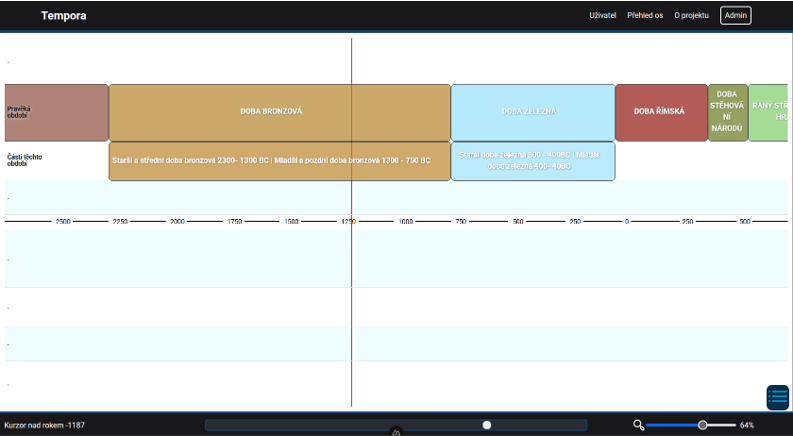
\includegraphics[width=1\linewidth]{Images/Detail-pravěk.png}
    \caption{Ukázka zobrazení přiblížené Pravěké osy }
    \label{fig:Detail-pravěk}
\end{figure}

\begin{figure}[h]
    \centering
    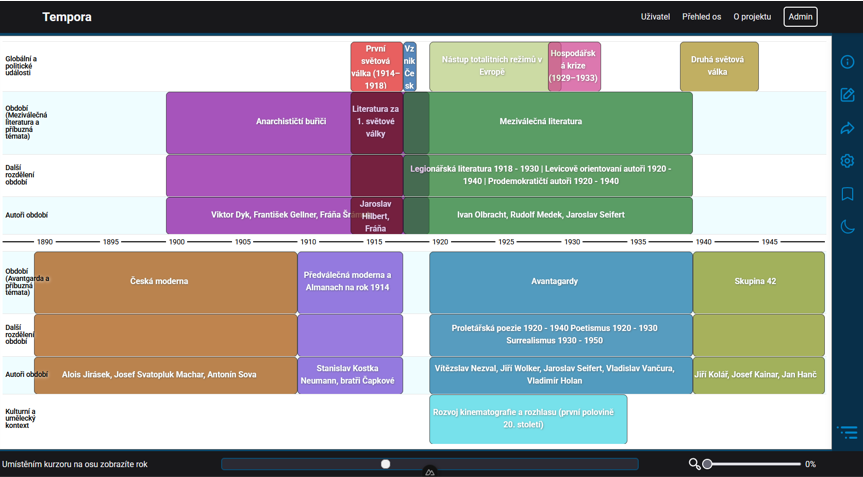
\includegraphics[width=1\linewidth]{Images/lit.png}
    \caption{Ukázka oddálené časové osy Literatura 20. století}
    \label{fig:lit}
\end{figure}

\begin{figure}[h]
    \centering
    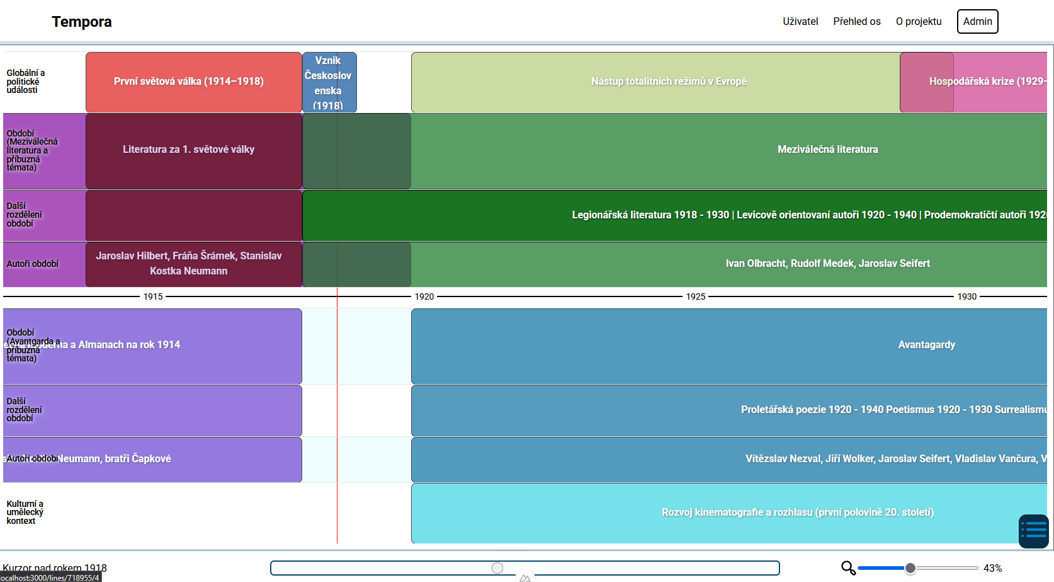
\includegraphics[width=1\linewidth]{Images/Detail-lit.png}
    \caption{Ukázka přiblížené časové osy Literatura 20. století}
    \label{fig:Detail-lit}
\end{figure}

\begin{figure}[h]
    \centering
    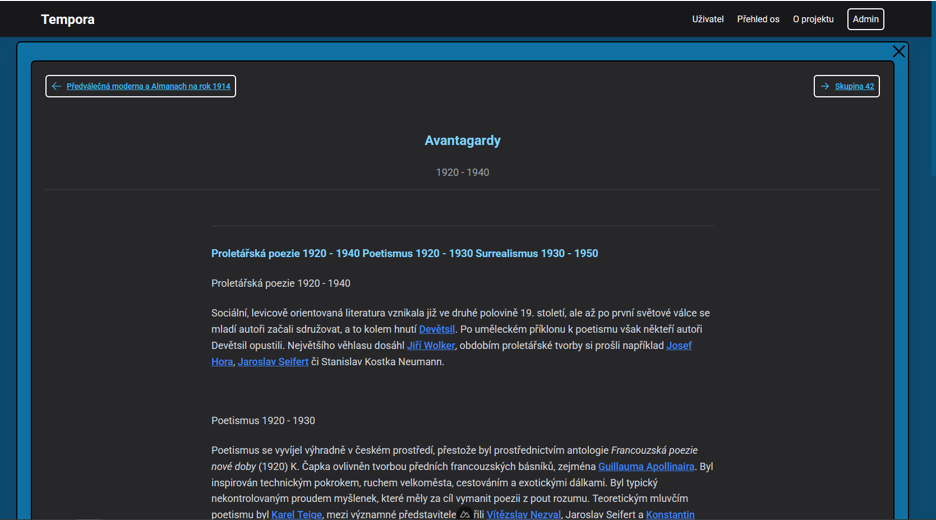
\includegraphics[width=1\linewidth]{Images/podrobnosti-lit.png}
    \caption{Ukázka zobrazení podrobností Avantgardy (tmavý režim)}
    \label{fig:podrobnosti-lit}
\end{figure}

\begin{figure}[h]
    \centering
    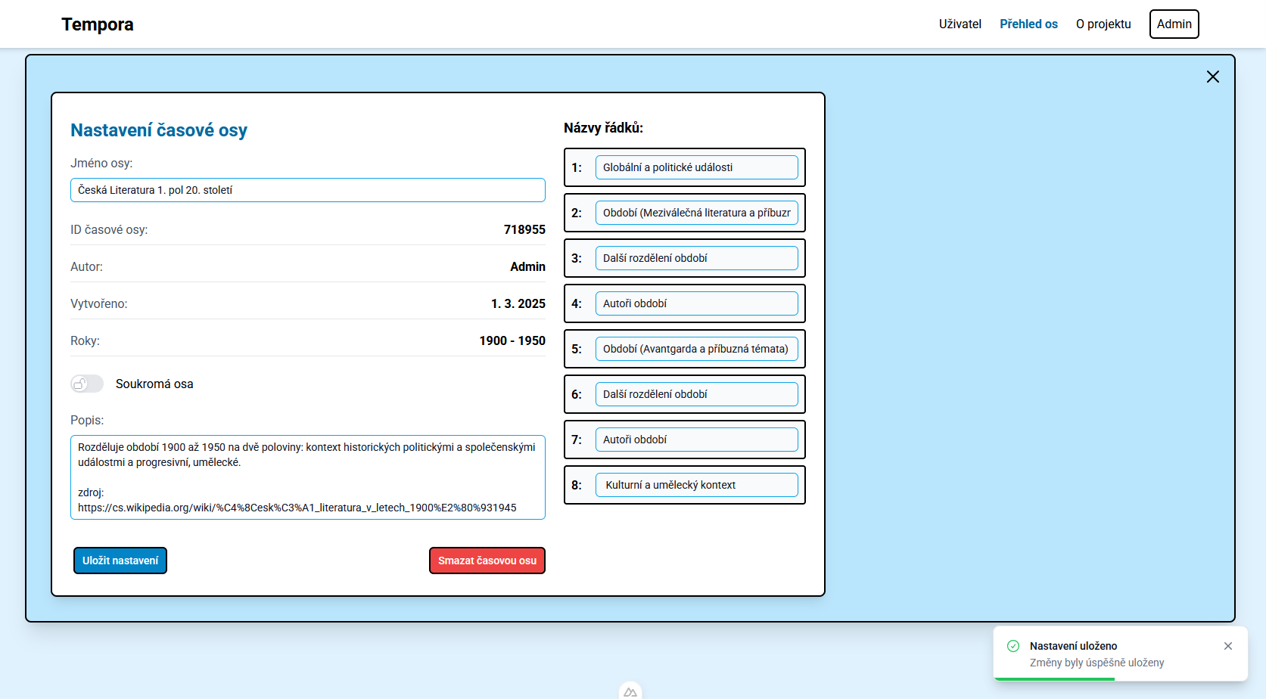
\includegraphics[width=1\linewidth]{Images/Settings.png}
    \caption{Ukázka možností nastavení časové osy s notifikací o uložení}
    \label{fig:Settings}
\end{figure}